\chapter{EVALUATION}

In this section we will evaluate the performance of the key components of the system, the Information Extraction module, the Ontology Similarity module, and the overall system resulting from the combination of the components.

\section{Experiments of Information Extraction }

To evaluate the performance of the information extraction module, we extract sentence types through the use of sentence filters. To explain the process of our experiment, we use the sentences whose content pertains to the applicant's college degree information.

In the experiment, we selected 100 sentences from existing job descriptions, and the content of these sentences were requirements of candidate degree and major. We labeled the values for "degree" and "major" manually. We use any content patterns that we can identify from these sentences to match and extract the degree information. Figure~\ref{fig:degree_accuracy} shows that when the total number of patterns increases, the accuracy of information increases as well. When we used 6 patterns, the accuracy of "degree" became 94\%. We also compared our pattern matching method to the conditional random field (CRF) model~\cite{lafferty2001conditional}, which is a state of art machine learning model for sequence labeling. We used 200 sentences to train the CRF model, and the features of the CRF model are words in the sentences and part of speech tags of the words. The accuracies of information extraction of the three fields with our two methods, pattern matching, and the application of the CRF model are shown in Table \ref{tab:ieaccura}

\begin{figure}[htbp]
  \centering
  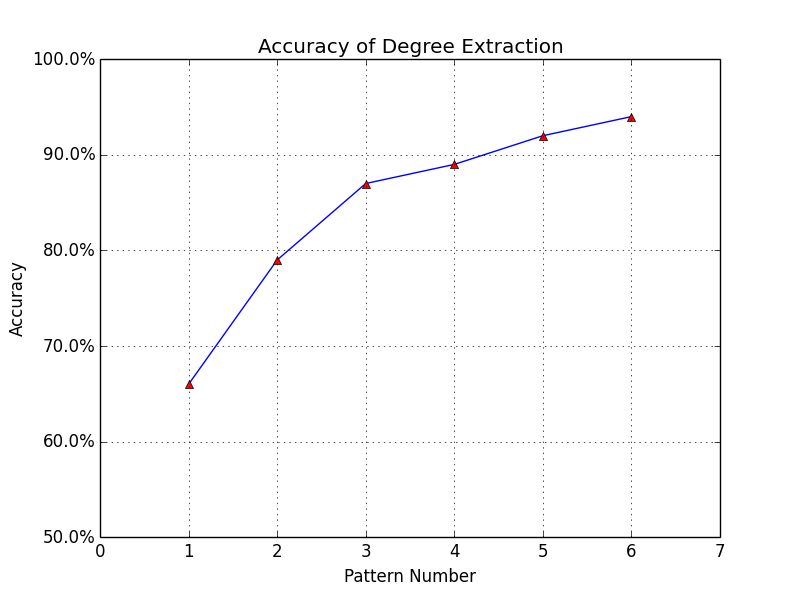
\includegraphics[scale=0.5]{images/degree_accuracy.png}
  \caption{Accuracy of Degree Extraction  }
  \label{fig:degree_accuracy}
\end{figure}


\begin{table}[ht]
\caption{Information Extraction} % title of Table
\centering % used for centering table
\begin{tabular}{   | c | c | c | c |   }
 \hline
          Field   & Pattern Num & Accuracy of Pattern Matching  & Accuracy of CRF   \\
 \hline
          Degree  & 6           & 0.94       &  0.85  \\
 \hline
          Major   & 10          & 0.85       &  0.72  \\
 \hline
          Skill   & 6           & 0.82       &  0.66  \\
 \hline
\end{tabular}
\label{tab:ieaccura} % is used to refer this table in the text
\end{table}

\section{Experiments of Ontology Similarity}

We selected some common skills from 500 job descriptions; table~\ref{tab:dismatrix3} shows similarity values between these skills. Higher values correspond to greater similarities, so the similarity between one skill and itself is 1. We selected one concept and ranked the other concepts by their similarity values to this concept. Human judges helped rank these concepts by assigning them "relevance scores" so that we can use NDCG to evaluate the effectiveness of our approach.

\begin{table}

\caption{Similarities of Skill List 1}
\begin{tabular}{ c | c c c c c c   }
 \hline
  Term       &  Java  &  JDBC  & Spring & Hibernate & MySql  & Oracle   \\  \hline
  Java   &   1    & 0.0523 & 0.091  &   0.0458  & 0.0339 & 0.0608    \\  \hline
    JDBC   & 0.0523 &   1    & 0.0525 &   0.0799  & 0.006  & 0.0616   \\  \hline
   Spring  & 0.091  & 0.0525 &   1    &   0.2008  & 0.0194 & 0.0878   \\  \hline
 Hibernate & 0.0458 & 0.0799 & 0.2008 &     1     & 0.0073 & 0.115    \\  \hline
   MySql   & 0.0339 & 0.006  & 0.0194 &   0.0073  &   1    & 0.049    \\  \hline
   Oracle  & 0.0608 & 0.0616 & 0.0878 &   0.115   & 0.049  &   1      \\  \hline
 \hline
\end{tabular}
\label{tab:dismatrix3}
\end{table}

We use the $ Normalized~Discounted~Cumulative~Gain ( NDCG )$ to evaluate the statistical-based similarity. NDCG is an important measure to evaluate the ranked retrieval results. For a set of queries $Q$, let $R(j,d)$ be the relevance score assessors given to a document $d$ for query $j$.
       $$ NDCG(Q,k) = \frac {1}{|Q|} \sum_{j=1}^{|Q|}{Z_{kj}} \sum_{m=1}^{k} \frac{2^{R(j,m)} - 1}{ \log_2(1+m)} $$

Where $Z_{kj}$ is a normalization factor calculated such that a perfect ranking's NDCG at $k$ for query $j$ is 1. For queries for which $k' < k$ documents are retrieved, the last summation is done up to $k'$.

Table~\ref{tab:simcompare1} shows how we evaluate the similarity between the concept ``Javascript'' and other concepts. The first column is a skill name, the second column is its similarity value to ``Javascript'', the third column is its position ranked by the similarity value, and the fourth column is its relevance value given by the judges. The NDCG value for concept Javascript is 0.94, and in Table~\ref{tab:simcompare2},  NDCG value for concept HTML is 0.97.

\begin{table}
\centering
\caption{ Javascript Similarity Evaluation : NDCG = 0.94 }
\begin{tabular}{ | c | c | c  | c |  }
 \hline
    Term     &  Similarity Value  &  Position   & Relevance     \\  \hline
    jQuery   &  0.1981            &      4      &   8        \\
     HTML    &  0.2087            &      3      &   4         \\
     CSS     &  0.2439            &      2      &   3   \\
     Java    &  0.0665            &      5      &   1   \\
    Python   &  0.0189            &      8      &   1   \\
     Ruby    &  0.023             &      7      &   1    \\
     JSP     &  0.0253            &      6      &   2    \\
 \hline
\end{tabular}
\label{tab:simcompare1}
\end{table}


\begin{table}
\centering
\caption{ HTML Similarity Evaluation : NDCG = 0.97 }
\begin{tabular}{ | c | c | c  | c |  }
 \hline
    Term      &  Similarity Value  &  Position   & Relevance     \\  \hline
  Javascript   &  0.2087           &      2      &   3        \\
     jQuery    &  0.0979           &      3      &   3         \\
     CSS     &  0.3569             &      1      &   5   \\
     Java    &  0.0473             &      4      &   1   \\
    Python   &  0.0175             &      6      &   1   \\
     Ruby    &  0.023              &      5      &   1    \\
     JSP     &  0.0103             &      7      &   3    \\
 \hline
\end{tabular}
\label{tab:simcompare2}
\end{table}


\section{Evaluation of the System}

In a traditional information retrieval systems, precision and NDCG are widely used measures~\cite{manning2008introduction}. Precision ($P$) is the fraction of retrieved documents that are relevant.
       $$  Precision =  \frac{ \#(releveant~items~ retrieved)}{ \#(retrieved~items)}$$

We first used Precision@K to compare the performance of our approach to the classical information retrieval models: Okapi BM25~\cite{robertson2009probabilistic}, Kullback-Leibler divergence, and the TF-IDF. Precision@K is the proportion of relevant documents in the first K positions and is given below:
$$ P@k = \frac{1}{k} \sum^m_{i=1} l_i 1 \left(  r(i) \leq k  \right )  $$
Where 1 is the indicator function: $1(A) = 1$ if A is true, 0 otherwise.

To evaluate a job finding, we compare the results of the system with three classical information retrieval models: Kullback-Leibler divergence~\cite{zhai2008statistical},  TF-IDF~\cite{manning2008introduction} and Okapi BM25~\cite{robertson1995okapi}. We give the definition of these measures below.

Kullback-Leibler divergence is a non-symmetric measure of the difference between two probability distributions $P$ and $Q$. The score of a document $D$ with respect to query $Q$ is given by:
\begin{equation}
    \begin{array}{rcl}
        s(D,Q) & = & -D( \theta_Q \parallel  \theta_D )\\
               & = &- \sum_{ \omega \in V } p (\omega \mid \theta_Q) \log \frac{ p (\omega \mid \theta_Q )}{p(\omega \mid \theta_D)} \\
               & = & \sum_{ \omega \in V } p (\omega \mid \theta_Q) \log p (\omega \mid \theta_D ) -  \sum_{ \omega \in V } p (\omega \mid \theta_Q) \log p (\omega \mid \theta_Q )  \\

    \end{array}
\end{equation}

In the equation $\theta_Q$ is the language model for a query, and  $\theta_D$ is the language model for a document.

TF-IDF is a Vector Space Model, which calculates the Cosine Similarity between the vectors of the query $q$ and the document $d$. In the equation, $tf$ is the term frequency, and $idf$ is the inverse document frequency. The TF-IDF weighting scheme assigned to term $t$ a weight in document $d$ given by:
$$ tf\text{-}idf_{t,d} = tf_{t,d} \times idf_{t} $$
The similarity between the query $q$ and the document $d$ given by:
$$ score(q,d) =  \sum_{t \in q }  tf\text{-}idf_{t,d} $$

Okapi BM25: Given a query $Q$, containing the keywords $q_1, ..., q_n$, the BM25 score of a document $D$ is:

$ score(D,Q) = \sum_{ i=1 }^{n} IDF(q_i) \cdot   \frac {f(q_i,D) \cdot (k_1 + 1)}{f(q_i,D) + k_1 \cdot ( 1-b + b\cdot \frac { \left | D \right |}{avgdl})}  $

In the evaluation phase, we created a data set of 100 job descriptions that includes several kinds of jobs such as web developers, server back-end developers, mobile developers and so on. We used 5 candidate r\'esum\'es and retrieved the top 20 jobs.  The relevance value of the job descriptions to each r\'esum\'e were set manually. We created a query q from the r\'esum\'e, treated the text of the job descriptions as documents d, and applied standard ad-hoc retrieval techniques to rank the jobs. We intended to return jobs that better matched the candidates' r\'esum\'es at the top. The result of Precision@k is in table~\ref{tab:job_precision}.


\begin{table}[ht]
\caption{Precision of Job Ranking } % title of Table
\centering % used for centering table
\begin{tabular}{    | c | c | c | c | c |  }
 \hline
       k     & Okapi BM25 & KL    & TF-IDF   & Ontology Similarity  \\
 \hline
       5     & 0.66       & 0.27  & 0.72     & 0.82   \\
 \hline
       10    & 0.46       & 0.27  & 0.50     & 0.76   \\
 \hline
       20    & 0.33       & 0.21  & 0.35     & 0.77   \\
 \hline

\end{tabular}
\label{tab:job_precision} % is used to refer this table in the text
\end{table}

The other measure we used is NDCG, which is explained in last section. Table~\ref{tab:job_ndcg} shows the NDCG value get from different information retrieval models. The result shows that Ontology Similarity  performs the best.

\begin{table}[ht]
\caption{NDCG of Job Ranking } % title of Table
\centering % used for centering table
\begin{tabular}{    | c | c | c | c | c |  }
 \hline
       k    & Okapi BM25 & KL    & TF-IDF & Ontology Similarity  \\
 \hline
       5    & 0.15       & 0.34  & 0.45     & 0.78   \\
 \hline
       10   & 0.18       & 0.44  & 0.47     & 0.72   \\
 \hline
       20   & 0.19       & 0.35  & 0.45     & 0.66   \\
 \hline

\end{tabular}
\label{tab:job_ndcg} % is used to refer this table in the text
\end{table}

